\chapter{Background}
\label{ch2_background}

\section{FPGA for Heterogeneous System}
The heterogeneous computing platform combines the traditional CPUs and additional compute architectures to accelerate computationally intensive tasks \cite{2}. Some of the examples are GPUs, MPPAs, Floating point units and cryptographic processors. This promises a new way for improving energy efficient systems. Accelerating tasks on MPPAs achieves better energy efficient solutions compared to GPUs and CPUs \cite{3}\cite{4}\cite{5}\cite{6}. The application specific design methodology provides another preferred approach to increase efficiency in area, power and speed. But increased time to market and associativity to higher costs hinders the ASIC design deployment.

FPGAs are the most preferred choice for rapid-prototyping the application specific accelerators in heterogeneous system architecture. It also provides flexibility to modify the hosted accelerator even after deployment \cite{7}\cite{8}\cite{9}. The new era of FPGA consists of Configurable Logic blocks (CLBs) connected by I/Os with the additional hard blocks called macros such as DSP blocks and reconfigurable embedded memories like BRAMs. The main concern in reconfigurable architecture is data transfer bandwidth and to use the hardware resources efficiently for the accelerator. Vendor specific hard processors are proposed \cite{10} to provide high bandwidth transfer. With hardware-software partitioning for an application, the hardware tasks are mapped to FPGA fabric using Hardware Description Languages(HDL) like Verilog and VHDL. For rapid design space exploration and to increase marginal performance in area and cost, the next preferred design method must be raising the level of programming abstraction. For example, Vivado HLS, a commercial tool from Xilinx, converts the C algorithmic implementation to RTL code.  

\section{Xilinx Zynq Zedboard}
Xilinx gave their new series of All-Programmable System on Chip (SoC) called Zynq which is a flexible and convincing platform for varied applications. It has a combination of ARM Cortex-A9 processor with FPGA, where these partitions are called as Processing System (PS) and Programmable Logic (PL) parts. Processing system can run a complete Linux Operating System and the programmable logic part can be configured with desired design. The Zynq architecture has a high bandwidth, low latency interfaces between PS and PL. Thus, Zynq platform enables the main processor to control the programmable hardware, which runs high intensive compute applications. Based on Zynq-7000 All-Programmable System on Chip, Xilinx has released a development and evaluation board called Zynq Zedboard. Zedboard consist of Zynq Z7020-clg484 of speed grade -1(MHz) package, which has ARM Cortex-A9 as an application processor for Processing System and reconfigurable fabric. The Processing System has 512MB DDR RAM, hard DMA Controller and double precision floating point unit with common peripherals and memory interfaces. Block diagram of PS is shown in Figure \ref{fig:1}\cite{11}. The main components of the PS are as below

\begin{itemize}\itemsep0em 
	\item Based on ARMv7 ISA, run-time configurable two ARM Cortex-A9 multicore processors.
	\item Neon 128b SIMD coprocessor and VFPv3 per processor.
	\item 32KB instruction and L1 data caches per processor.
	\item 512KB L2 cache that is shared between the processors.
	\item Snoop Control Unit (SCU) and the ACP for cache coherent accesses.
	\item On-Chip Memory (OCM) with capacity of 256KB.
	\item DDR controller comprising of AXI memory port interface, digital PHY and transaction scheduler.
	\item DMA controller with four channels for PS and PL.
\end{itemize}
\begin{figure}[h]
    \centering
    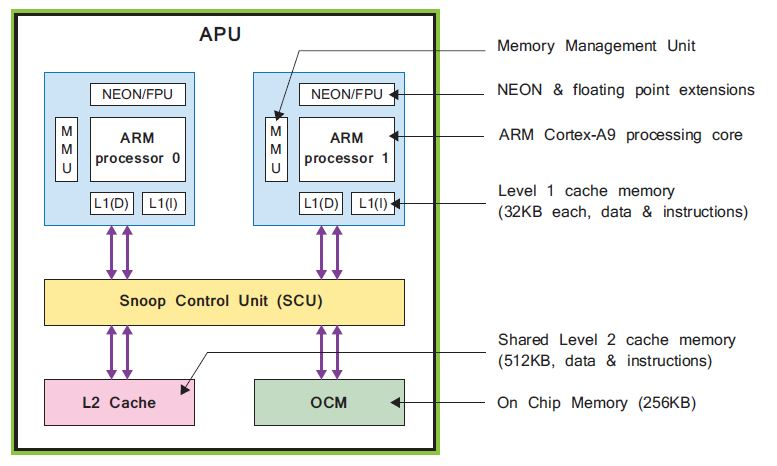
\includegraphics[width=0.90\textwidth]{Processing_system}
    \caption{Block Diagram of Processing System}
    \label{fig:1}
\end{figure}

The programmable logic part is made up of Artix 7 FPGA fabric. The PL can be configured partially or fully with the configuration data as a bitstream. The PL power can be managed for real time applications. The configurations of PL are listed below \cite{23}.

\begin{itemize}\itemsep0em 
	\item 36KB block RAM with capability of dual port.
	\item DSP48E1 Slice with optional pipelining, ALU and dedicated buses for cascading useful for Digital signal processing.
	\item Low jitter clock distribution and low skew.
	\item High performance I/O that can be configured.
	\item Dual Analog-to-Digital Converter (ADC) blocks with 12-bit and 1 MSPS rate.
\end{itemize}

The Zynq platform uses multiple AXI channels for communication between PS and PL. There are three types of AXI interfaces shown below.
\begin{itemize}\itemsep0em 
	\item Two 32-bit, AXI master and slave general purpose ports -- AXI\_GP.
	\item Four 32/64-bit, AXI slave high performance ports -- AXI\_HP.
	\item One 64-bit configurable, AXI slave Accelerator Coherency Port -- AXI\_ACP.
\end{itemize}

\section{OpenCL}
Open Computing Language (OpenCL) is a framework for heterogeneous programming, managed by non-profit consortium Khronos group. OpenCL APIs are restricted version of C99 language that can be used for developing parallel code for various computing devices like CPUs, GPUs, Accelerated Processing Unit. OpenCL C Code is called as program, comprises of collection of functions called kernels. Kernels are the basic part of the OpenCL Program that executes on the device. OpenCL guides the programmer to develop OpenCL targeted parallel program. It offers both Host management layer and Device layer. Host management layer or a host program is executed by the user and manages the number of devices in the system for kernel execution. While, Device layer is designed for mapping the parallel code to the selected device. OpenCL specification is categorized into four basic models. They are Platform model, Execution model, Memory model and Programming model.

\subsection{Platform Model}
The single host directs execution on one or more devices as shown in the figure \ref{fig:2}. Platforms are vendor specific implementation of OpenCL APIs. It is the abstract way of representing the devices in a heterogeneous system. Vendor maps the abstract architecture to physical hardware. In simple ways, if programmer chooses vendor A's platform, he cannot communicate vendor B's GPU in the same system.  The platform model defines the compute device as an array of compute units like some of the GPU model and each compute unit is further divided into processing elements (PE). The OpenCL API function clGetPlatformIDs() discovers the available number of platforms for a given system. The compute devices can be identified by clGetDeviceIDs() with following device types like CPU, GPU or Accelerator. The device\_type argument is used to limit the required devices for selection by a programmer.
\begin{figure}[h]
    \centering
    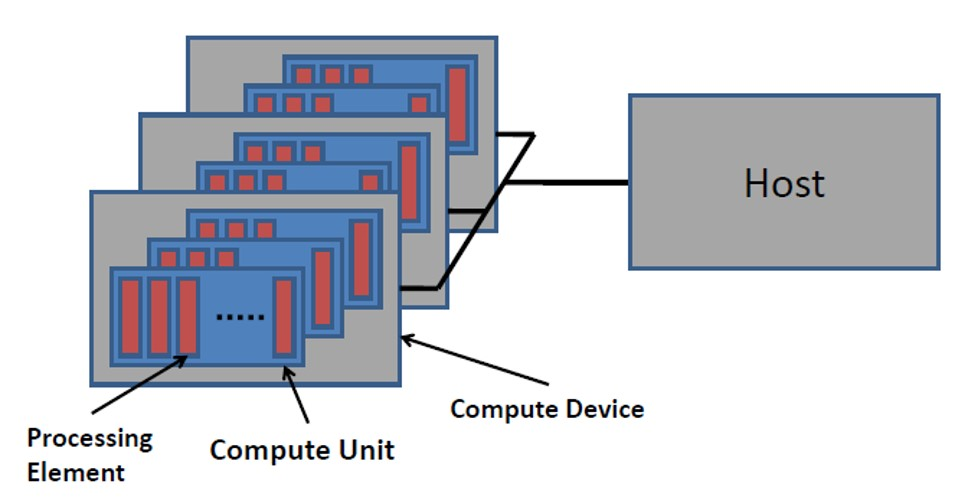
\includegraphics[width=0.80\textwidth]{Platform_Model}
    \caption{Platform Model}
    \label{fig:2}
\end{figure}

\subsection{Execution Model}
A context is created for managing the execution of OpenCL Commands, which includes data movement and kernel execution. A Kernel program is available as a source in ISO C99 standard with several extensions. Host program builds the kernel program to map accordingly to the device using clBuildProgram() API. A kernel instance is created for each index available, based on the index space for a device. Each kernel instance is called work item. Work item are the basic unit for concurrent execution. To facilitate the scalability, the work items in N -- dimensional range is divided into equal work group sizes. It can be specified as one, two or three-dimensional vectors. Work group size is fixed to a specific group size for efficient hardware implementation. Work items are executed with the function call to clEnqueueNDRangeKernel().
\begin{figure}[h]
    \centering
    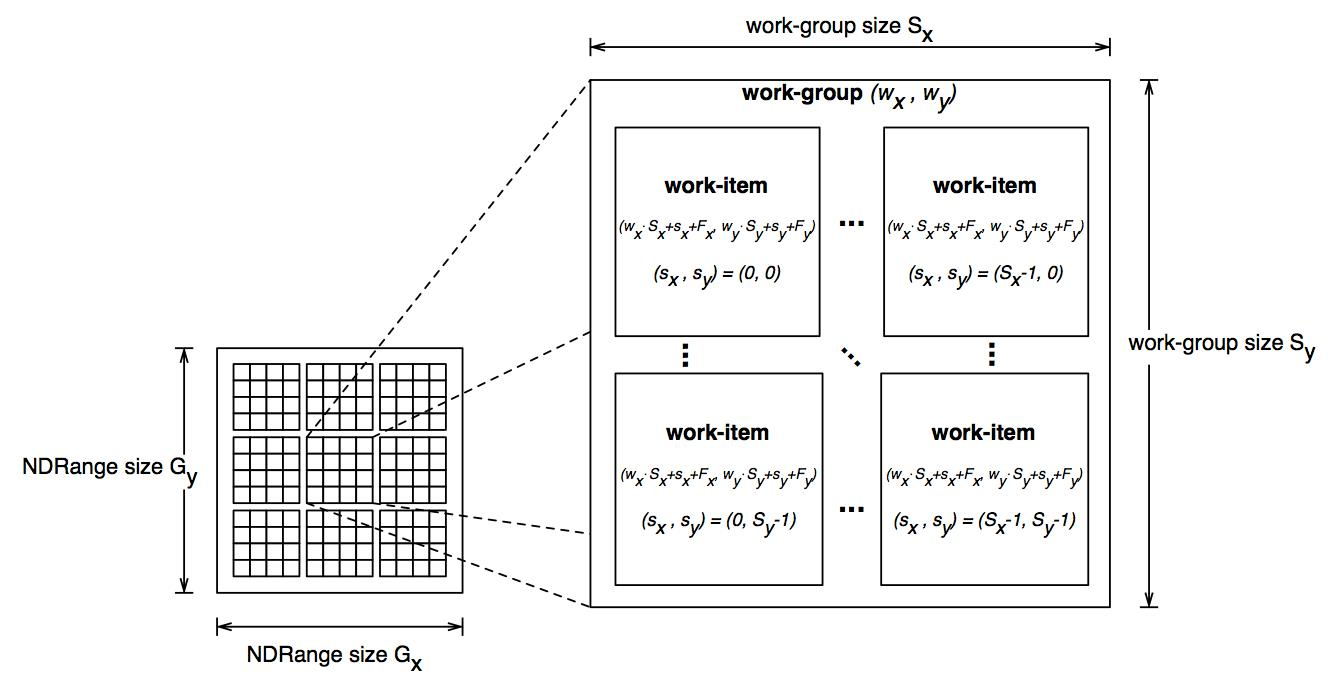
\includegraphics[width=1\textwidth]{execution_model}
    \caption{An Example of 2-dimensional index space}
    \label{fig:3}
\end{figure}

For Example, A hardware with two-dimensional index space has Gx by Gy work items. Figure \ref{fig:3} \cite{12} contains nine work groups with each of size Sx by Sy. Work-groups are assigned with an ID (wx, wy) and work items have local and global ID. Global ID are assigned using global offset called Fx and Fy. 

\subsection{Memory Model}
OpenCL defines an abstract model to map the memory space into hardware. Usually the memory subsystems differ between platforms. For example, CPU has automatic cache system while GPUs do not support. Thus, OpenCL C language provides four address spaces called private, local, global and constant. Programmer uses keywords to associate the memory space for variable. Global memory is visible to all compute units on the device. The initial data transfer from host to device will reside in global memory. Constant memory is accessed simultaneously by all the work items and it is designed for read only. Local memory is shared between work groups and it is unique for each compute device. Whereas Private memory is unique to an individual work items. The memory model of OpenCL is closely related to modern GPUs.

Hence, the platform model defines the host and device. The kernel creation and execution are set up by the hosts using execution model with required space for parallelism. Then data transfers and memory space are managed using memory model. Contexts and kernel are created and mapped using programming model. A typical OpenCL Implementation requires all the above model. The OpenCL runtime and driver will map the memory spaces to the physical hardware.

\section{Related Work}
LE1 \cite{13}, a customized VLIW chip multiprocessor is designed with unified compilation strategy. A LLVM compilation prototype was developed to enable the OpenCL application execution on LE1 CPU. The compilation flow automates the coalescing of work items for better utilization of cores available. LE1 provides super linear performance with certain improvements from compiler optimization.

An Accelerator based on $\uprho$--VEX Processor \cite{14} is implemented on ML605 Platform. The $\uprho$--vex processor is a VLIW processor instantiated on FPGA and it is interfaced to the host system using PCI Express Bus. To abstract the accelerator in software, OpenCL framework has been developed. The communication interface is developed as Linux kernel drivers, which is used as OpenCL Drivers. With the available LLVM backend for $\uprho$--Vex processor, a runtime support can be integrated in OpenCL framework. OpenCL drivers and runtime for accelerator are implemented using POCL's OpenCL framework. The key features are analyzing execution time with three main contributing factors. They are data transfer throughput, kernel compile time and kernel execution time. The proposed accelerator achieved 1.2 to 0.11 times the performance of modern GPUs.

Texas Instrument's System on Chip (ARM as host and DSP as device)\cite{15} and DSP device with PCI-E interface supports OpenCL framework. TI's Kernel compilation flow for OpenCL devices uses LLVM passes from POCL. It also supports both online and offline kernel compilation. With LLVM passes, the kernel functions or work items are transformed into work group functions.
